%%%%%%%%%%%%%%%%%%%%%%%%%%%%%%%%%%%%%%%%%%%%%%%%%%%%%%%%%%%%%%%%%%%%%
\begin{frame}{Motivating Scenarios}
    Fukushima Disaster (2011)
    %\footnote{https://rememberfukushima.org/fallout-maps/}
    \hspace{0.4 cm}
    Deep Water Horizon (2010)
    %\footnote{https://response.restoration.noaa.gov}
    \\
	\begin{minipage}{0.45\textwidth}	
		\begin{figure}
			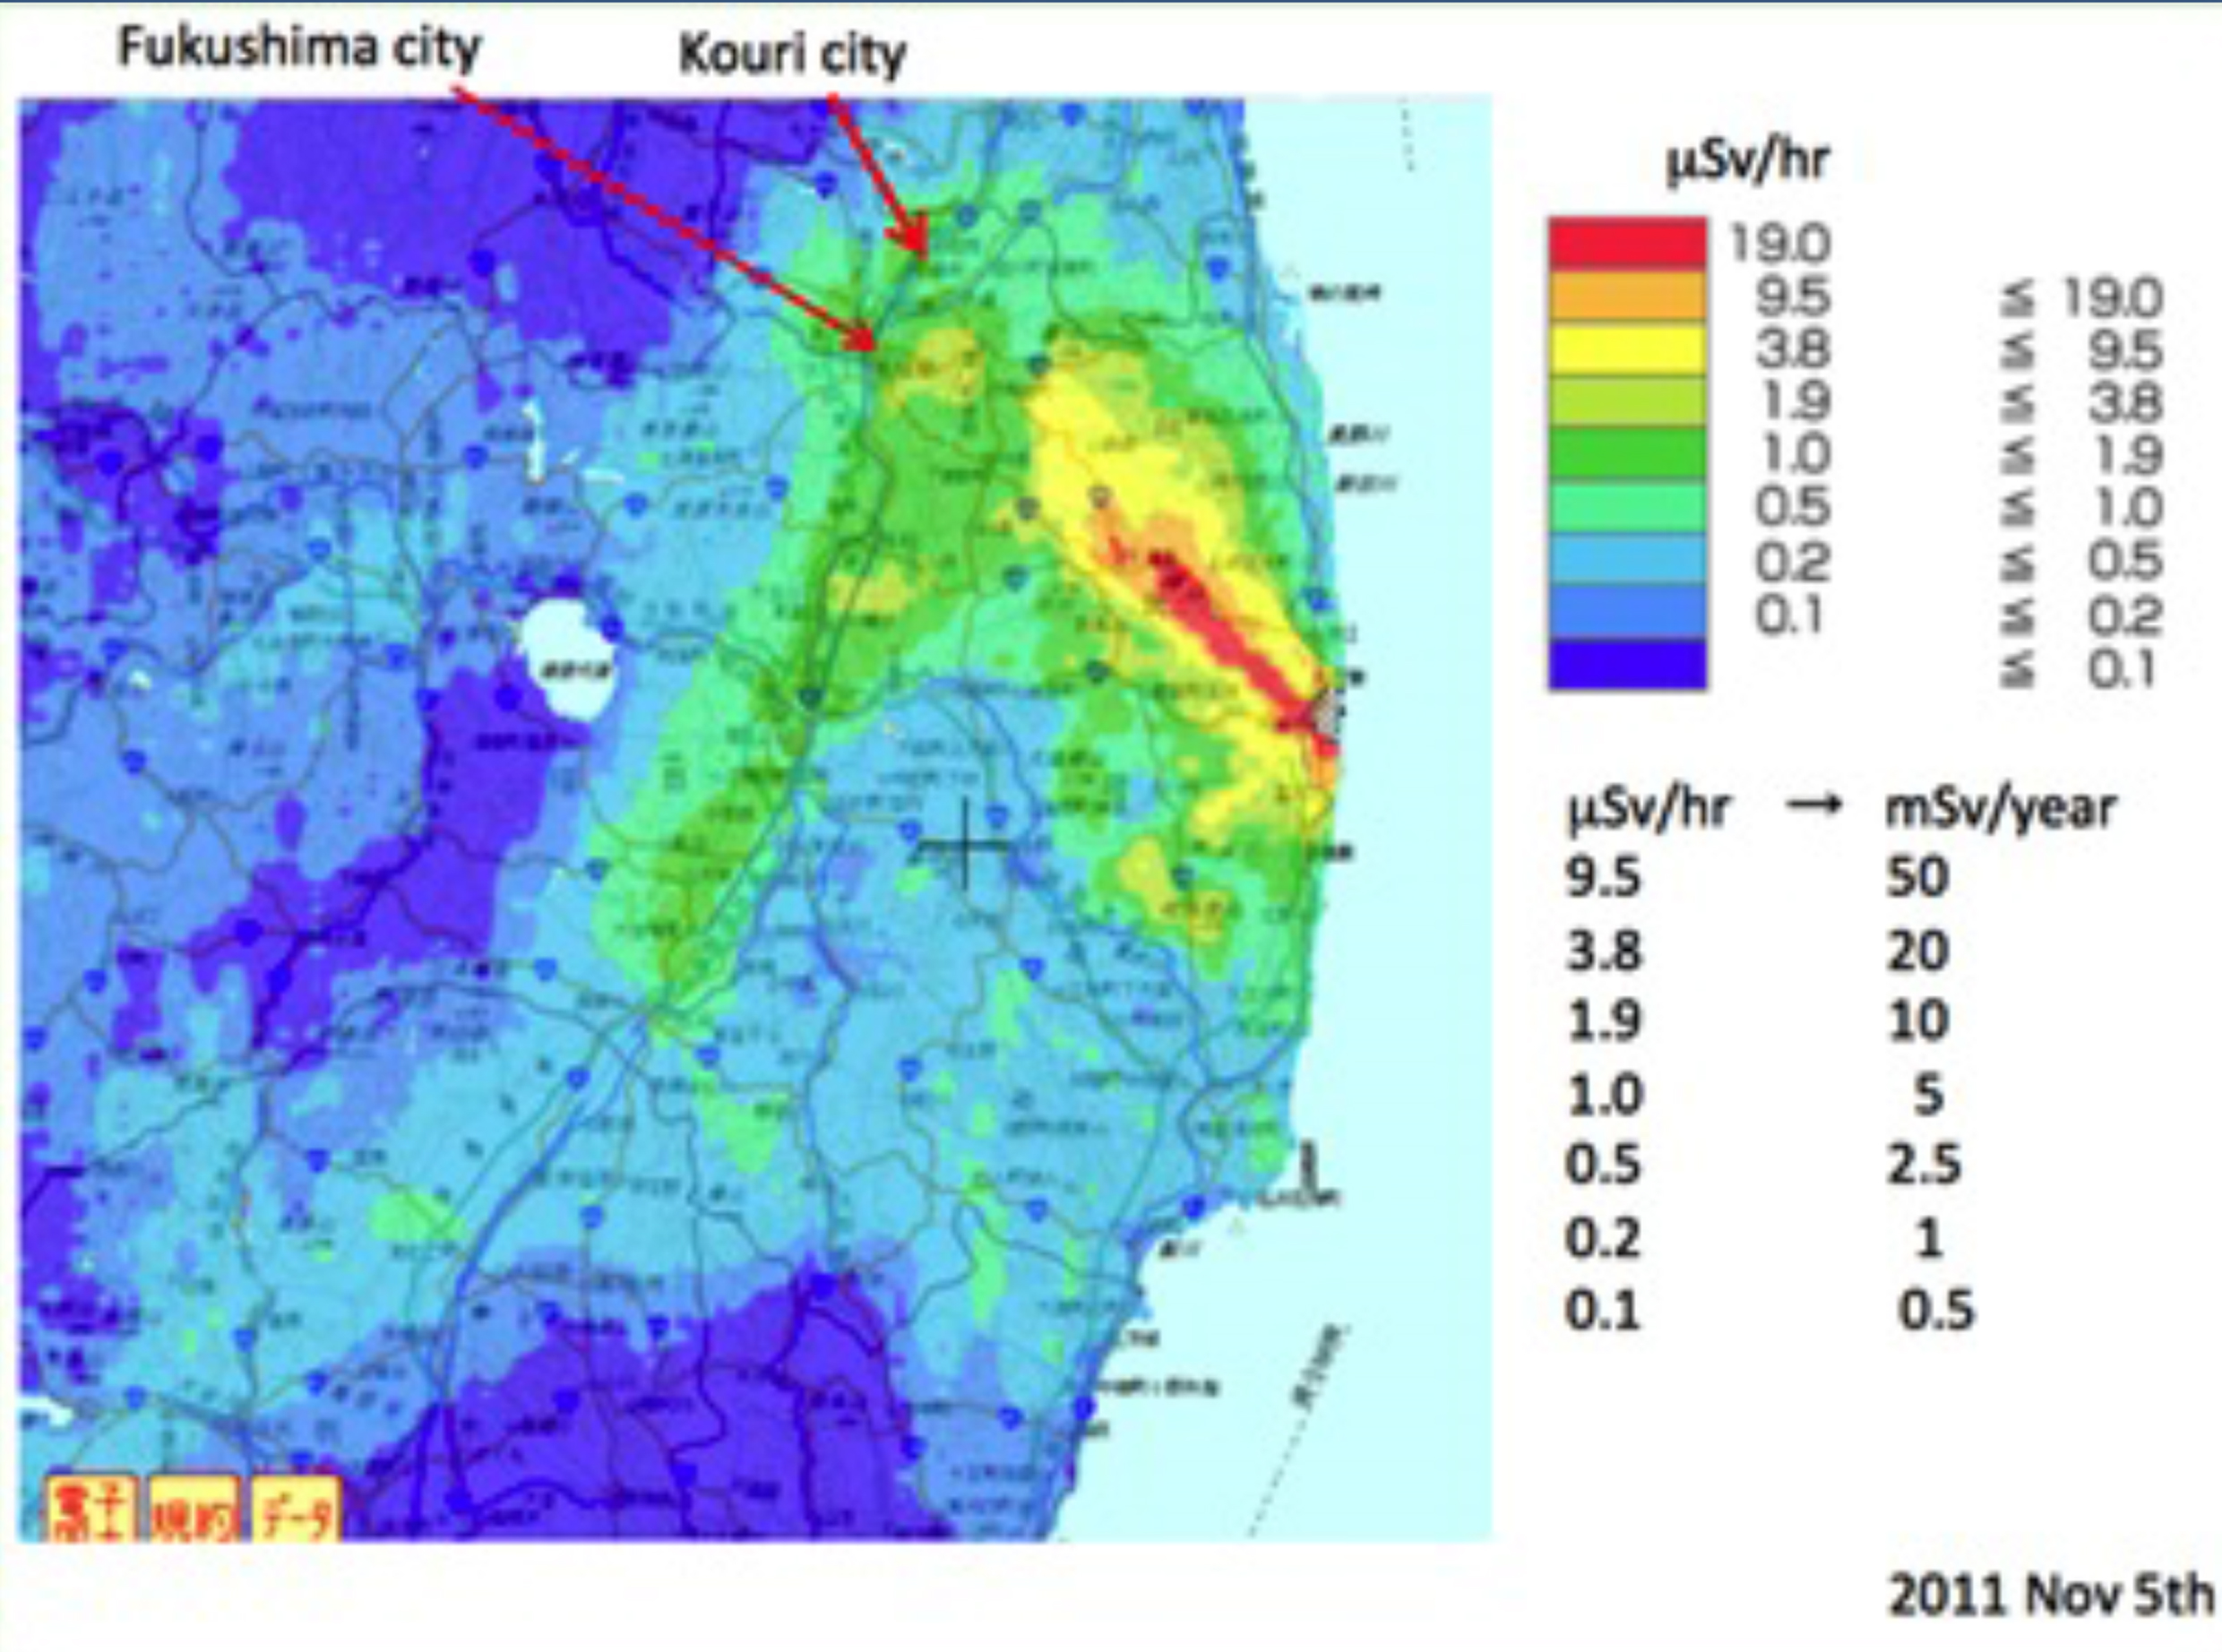
\includegraphics[width=1\textwidth]{figures/fukushima_disaster.jpg}
			%\caption{Fukushima Disaster (2011)}
			%\label{fig:fukushima_disaster}
		\end{figure}
		\begin{figure}
			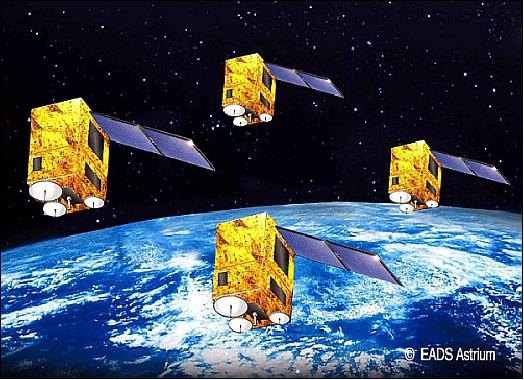
\includegraphics[scale=0.2]{figures/Essaim_constellation.jpg}\label{fig:satellite_flock}
		\end{figure}
	\end{minipage}
	\hspace{0.05cm}
	\begin{minipage}{0.45\textwidth}
		\begin{figure}
			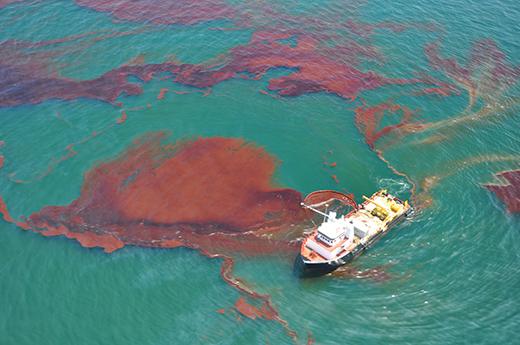
\includegraphics[width=\textwidth]{figures/oil_spill.jpg}
			%\caption{Oil Spills}
			%\label{fig:oilspills}
		\end{figure}
		\begin{figure}
			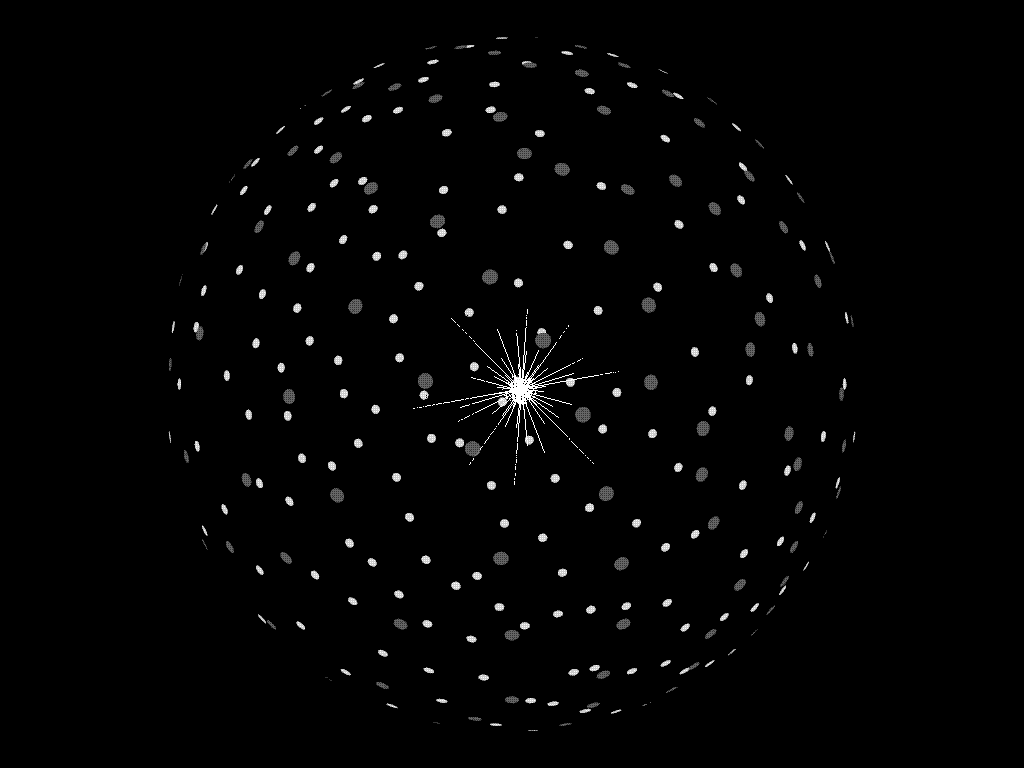
\includegraphics[scale=0.1]{figures/Dyson_swarm.png}		
			\label{fig:Dyson_swarms}
		\end{figure}	
	\end{minipage} 
 .
 \hspace{0.5 cm}
  EADS Astrium 
 %\footnote{https://earth.esa.int}
\hspace{1.7 cm}
Dyson Swarm (Why not !)
\\
\vspace{0.5cm}
\begin{itemize}
	\item Have figures for: Formation forming, flocking, source-seeking, Platooning 
\end{itemize}
\end{frame}
%%%%%%%%%%%%%%%%%%%%%%%%%%%%%%%%%%%%%%%%%%%%%%%%%%%%%%%%%%%%%%%%%%%%%
%%%%%%%%%%%%%%%%%%%%%%%%%%%%%%%%%%%%%%%%%%%%%%%%%%%%%%%%%%%%%%%%%%%%%
\begin{frame}{Physical Agent Dynamics}	
	\begin{itemize}
		\item Crazyflie picture 
		\item Hippo campus picture
		\item Zooids picture
		\item LTI/LPV agents, non-holonomic constraints
	\end{itemize}
\end{frame}
%%%%%%%%%%%%%%%%%%%%%%%%%%%%%%%%%%%%%%%%%%%%%%%%%%%%%%%%%%%%%%%%%%%%%
%%%%%%%%%%%%%%%%%%%%%%%%%%%%%%%%%%%%%%%%%%%%%%%%%%%%%%%%%%%%%%%%%%%%%
\begin{frame}{Core Idea}	
	\begin{itemize}
		\item Control of a single non-linear (possibly non-holonomic) agent: Well-studied problem and various techniques available
		\begin{itemize}
			\item LPV
			\item Dynamic-inversion
			\item Flatness-based control
		\end{itemize}		
		\item About three decades of work on studying interconnections of "simple" agent dynamics where simple could for example be
		\begin{itemize}
			\item single/ double integrators
			\item positive systems 
		\end{itemize} 
	\item Can we maintain this separation in the controller design? i.e design local agent controllers and study the interconnections of these closed loop systems
	\item Can we give some stability and performance guarantees with such a strategy?
	\item What kind of control architectures are possible?
	\end{itemize}
\end{frame}
%%%%%%%%%%%%%%%%%%%%%%%%%%%%%%%%%%%%%%%%%%%%%%%%%%%%%%%%%%%%%%%%%%%%%
%%%%%%%%%%%%%%%%%%%%%%%%%%%%%%%%%%%%%%%%%%%%%%%%%%%%%%%%%%%%%%%%%%%%%
\begin{frame}{Different Control Architectures}	
	\begin{minipage}{0.45\textwidth}	
		\begin{figure}
			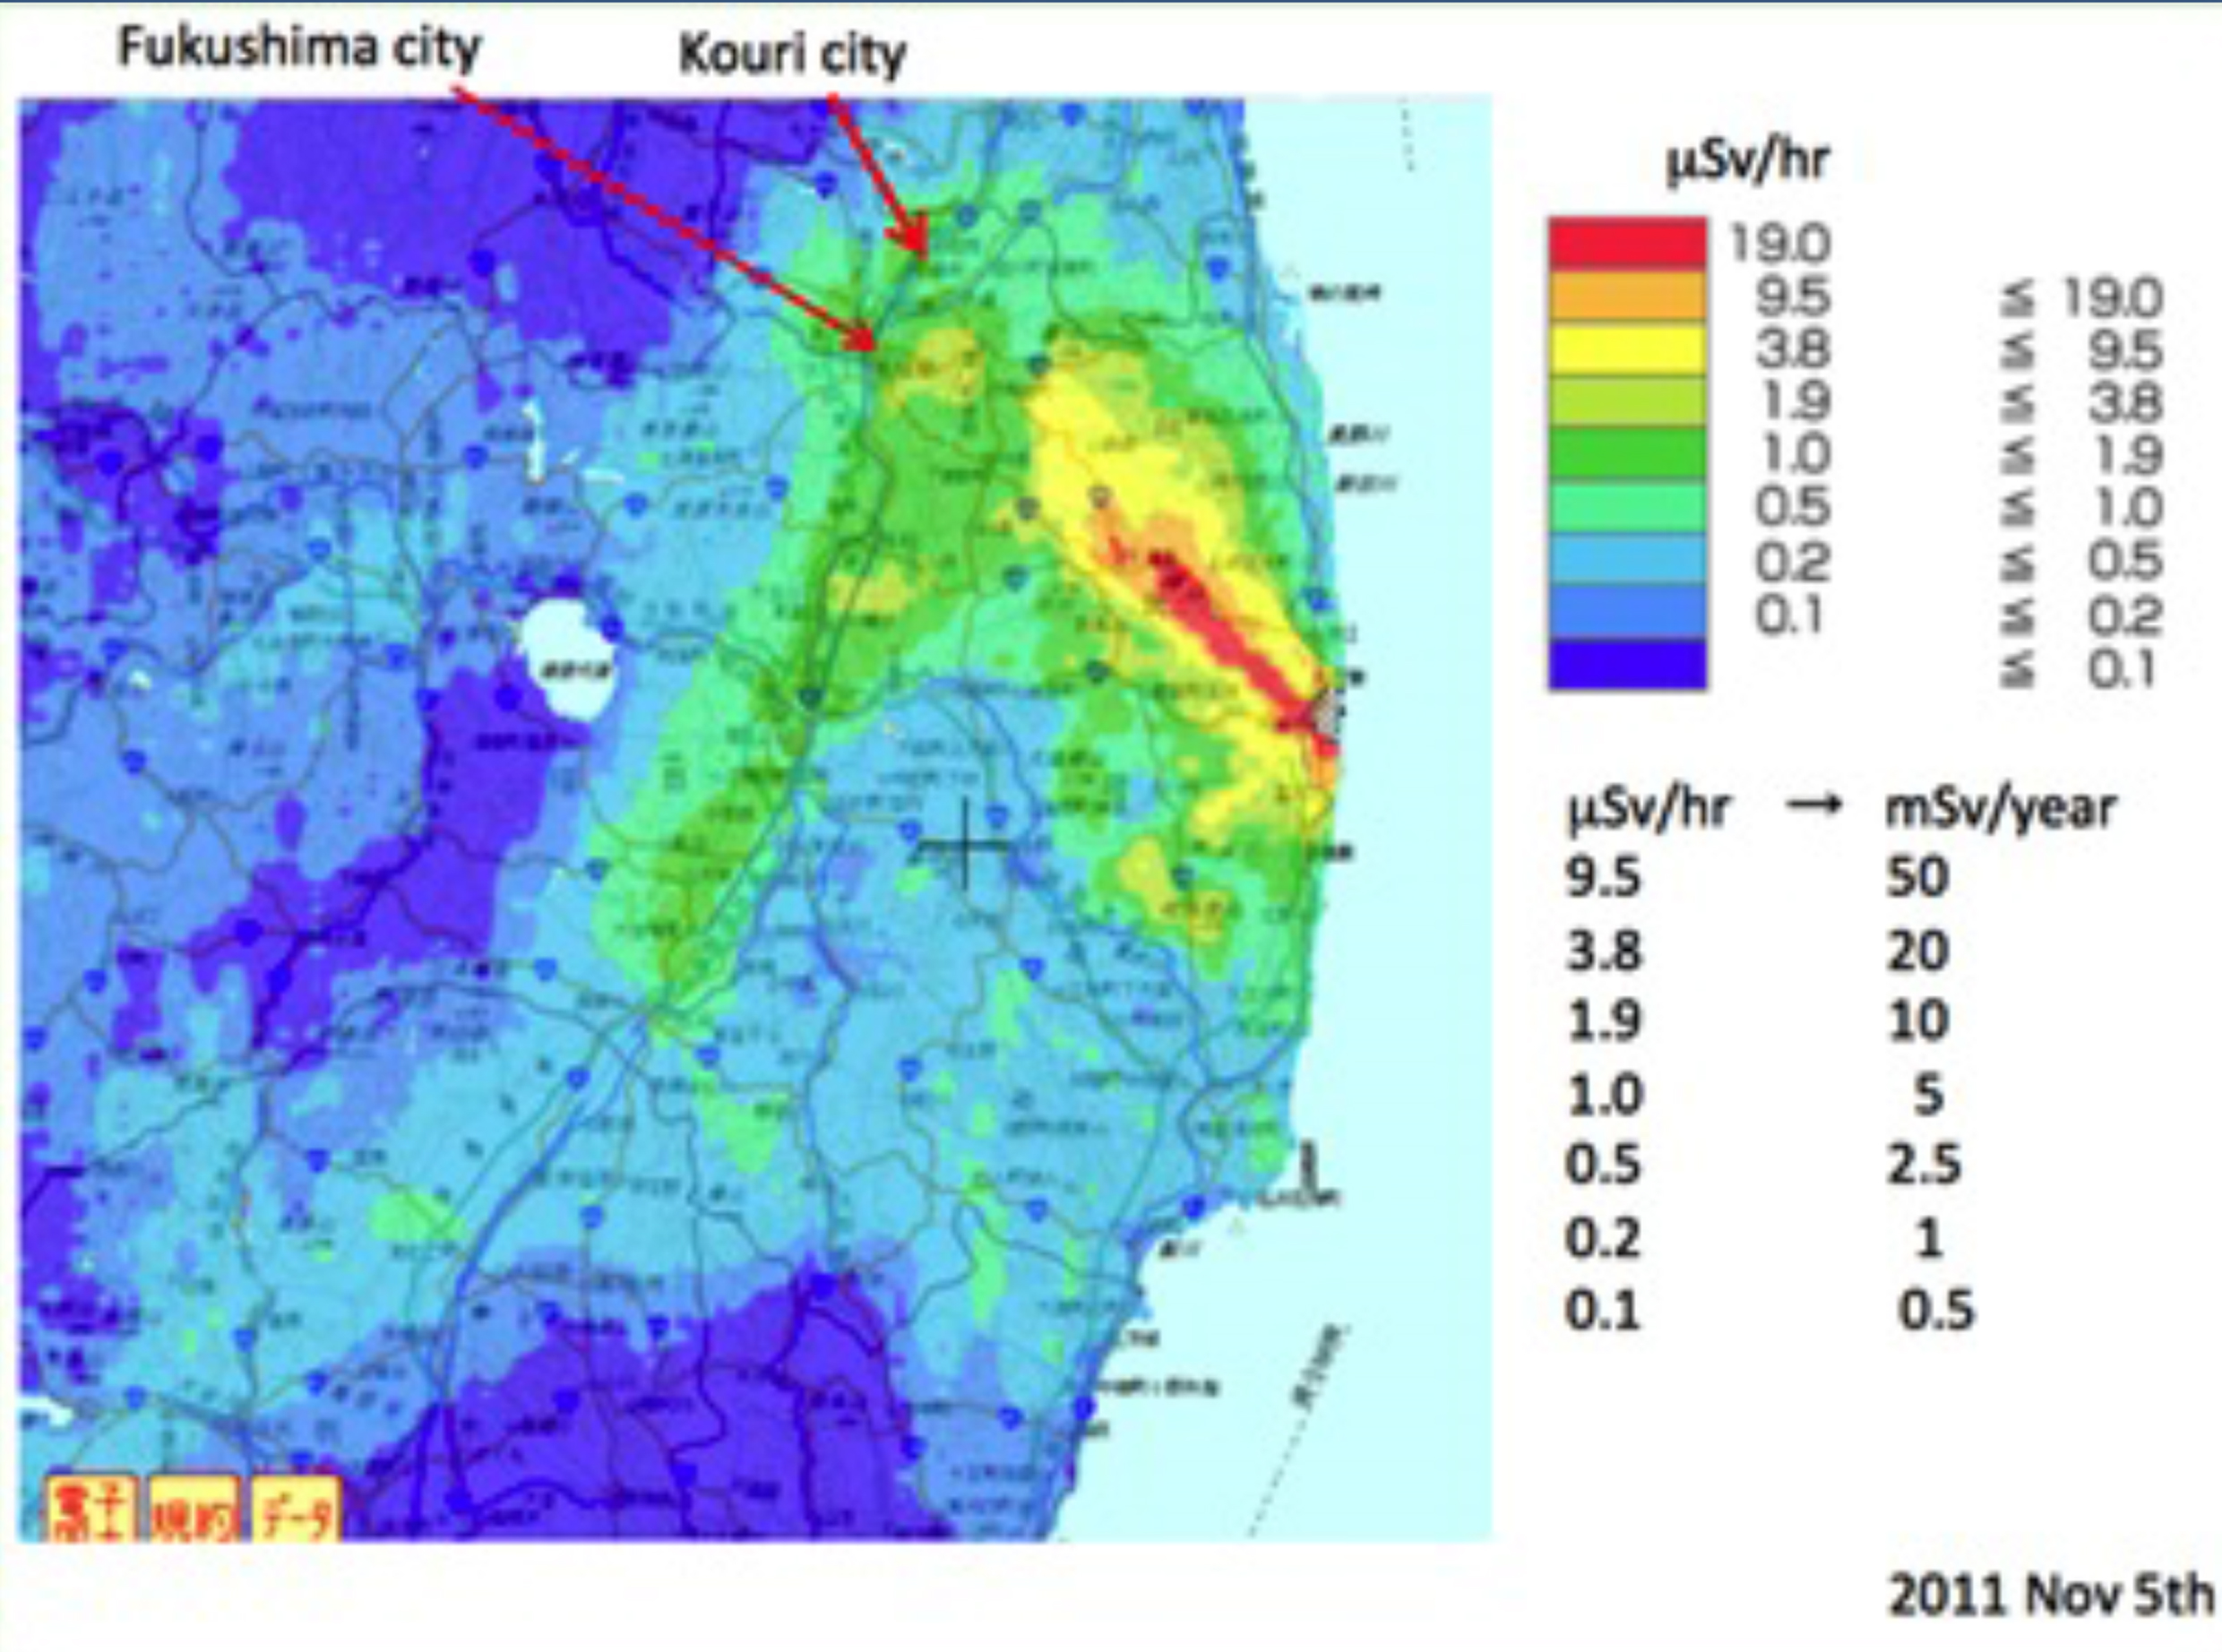
\includegraphics[width=1\textwidth]{figures/fukushima_disaster.jpg}
			%\caption{Fukushima Disaster (2011)}
			%\label{fig:fukushima_disaster}
		\end{figure}
		Coupled architecture
		\begin{itemize}
		\item Maintenance of relative positions important (e.g asdf) 
		\item inter-agent distances are low
		\item High disturbances
		\end{itemize}
	\end{minipage}
	\hspace{0.05cm}
	\begin{minipage}{0.45\textwidth}
			\begin{figure}
			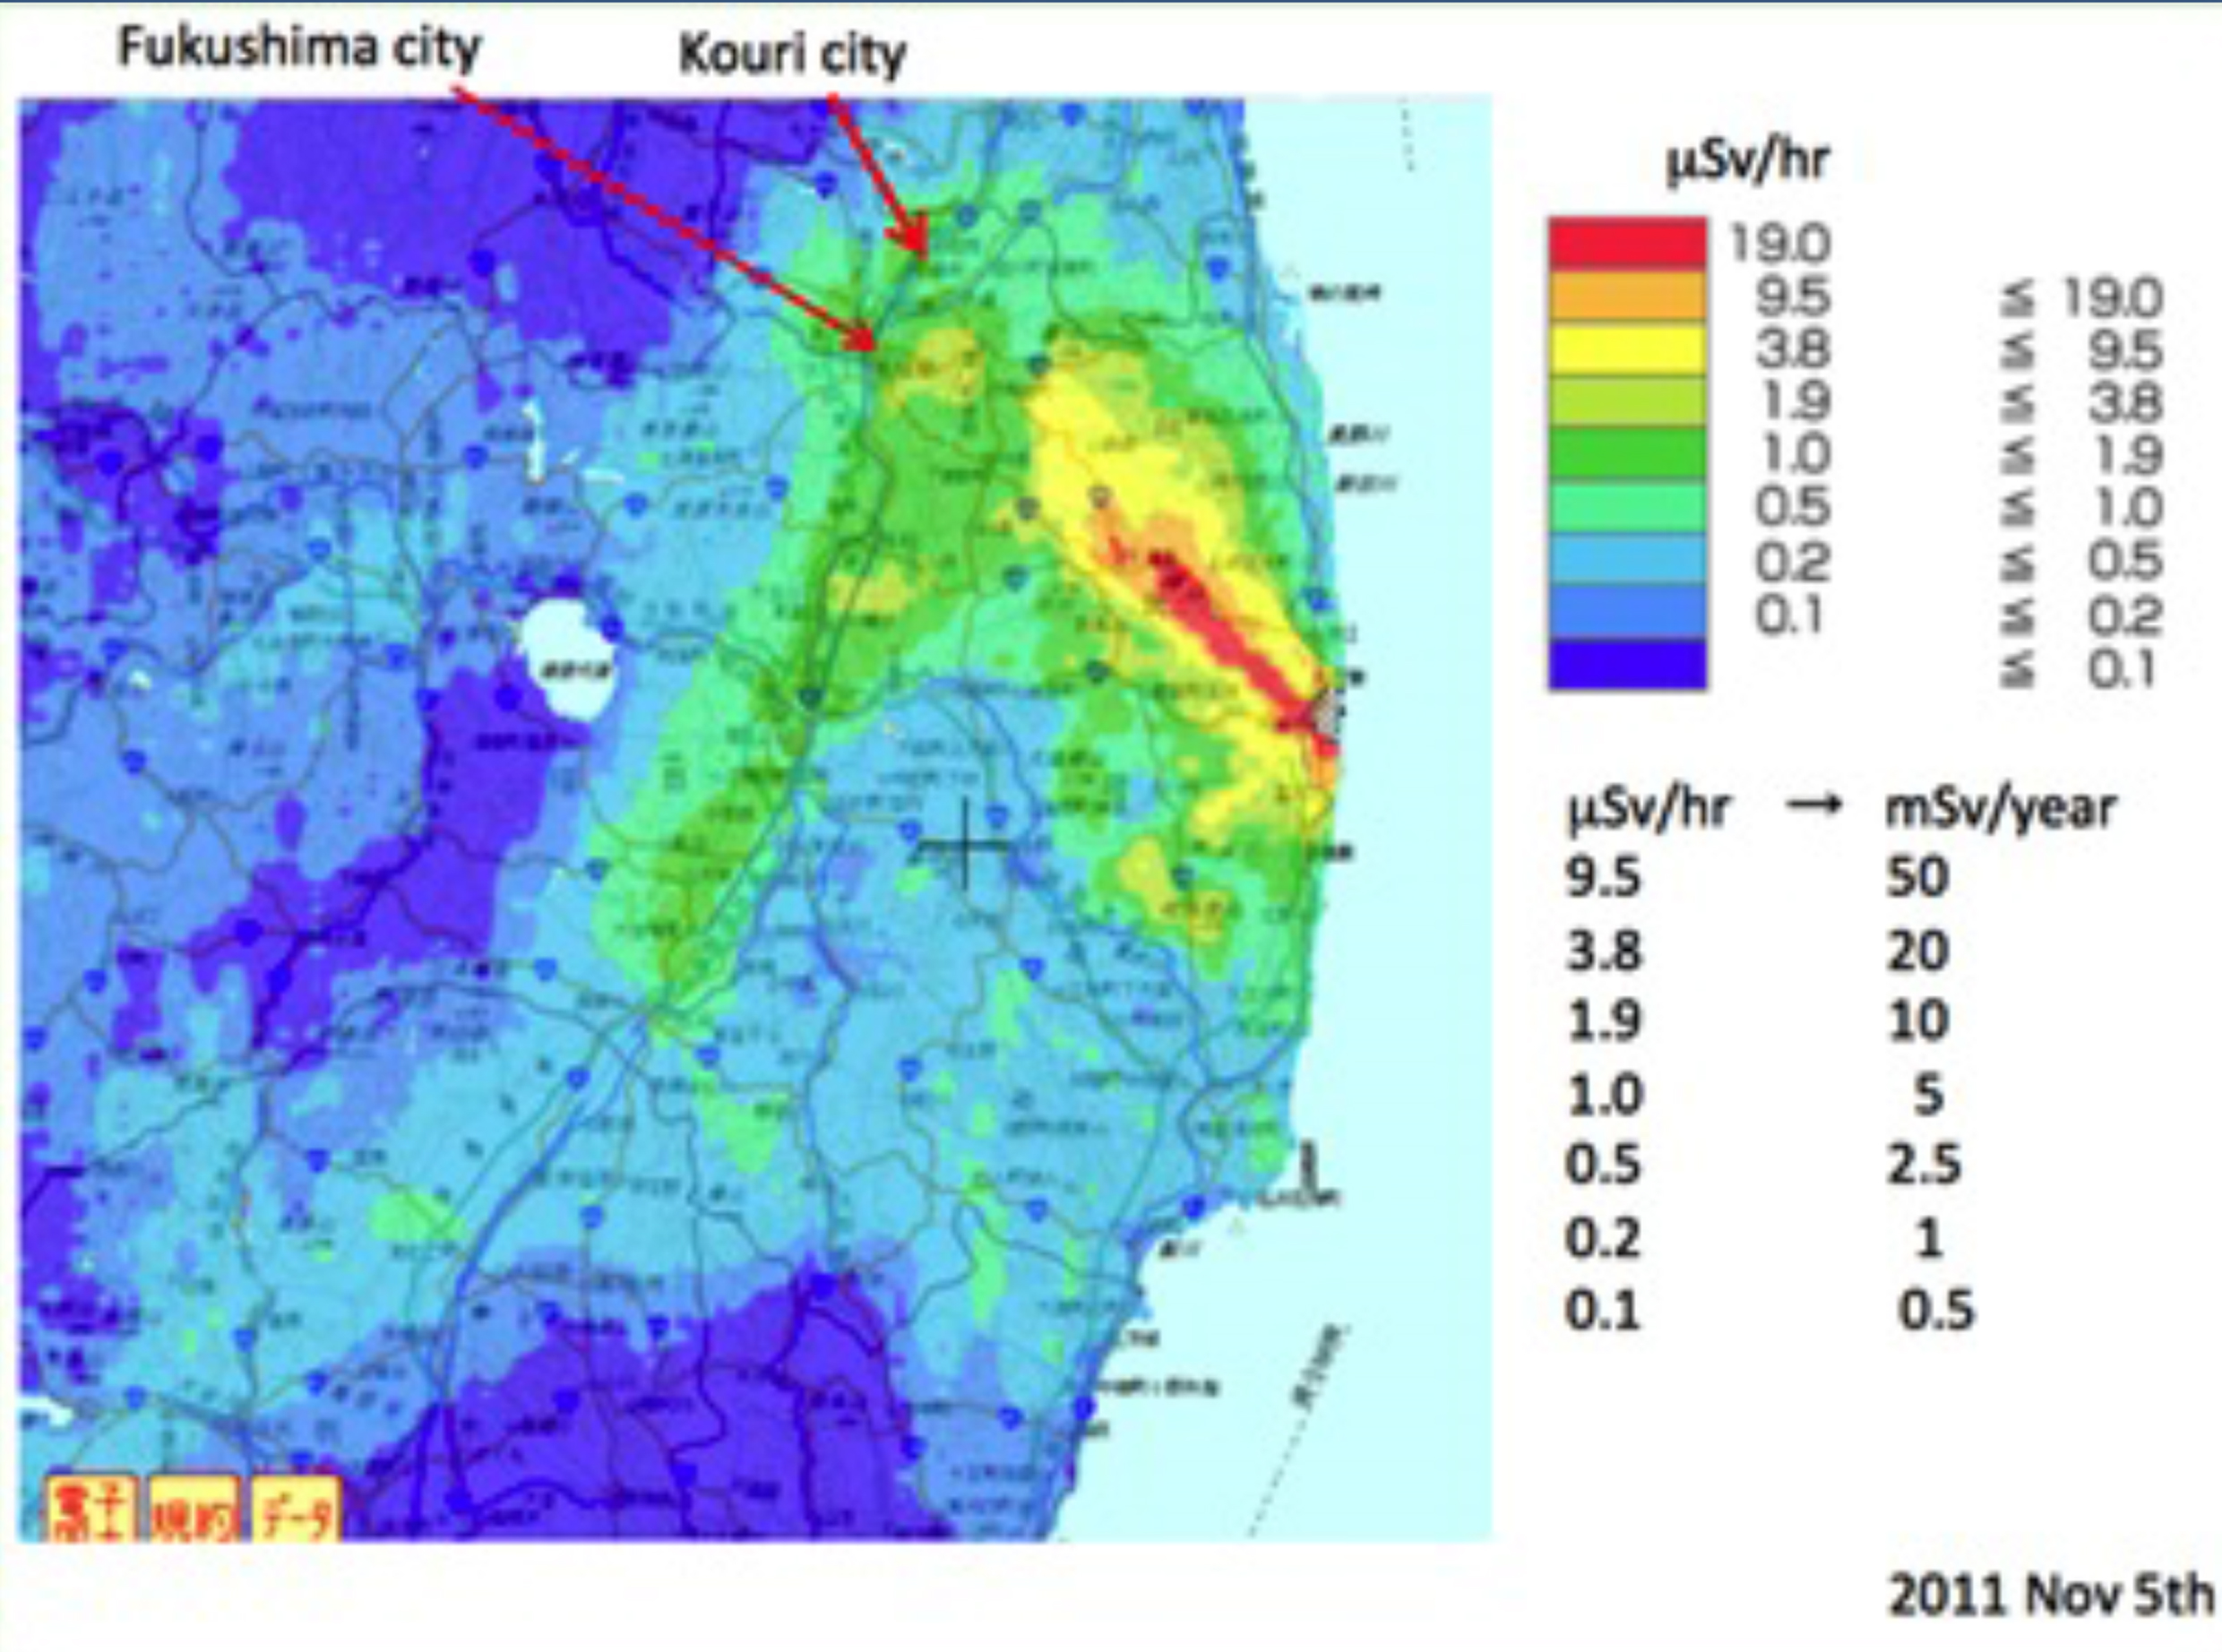
\includegraphics[width=1\textwidth]{figures/fukushima_disaster.jpg}
			%\caption{Fukushima Disaster (2011)}
			%\label{fig:fukushima_disaster}
		\end{figure}
		Coupled architecture
		\begin{itemize}
			\item Maintenance of relative positions important (e.g asdf) 
			\item inter-agent distances are low
			\item High disturbances
		\end{itemize}
	\end{minipage} 
	\begin{itemize}
		\item Combination of the two		
	\end{itemize}
\end{frame}